\chapter{Kontrollieren} \label{ch:check}

In diesem Kapitel wird das Endprodukt auf seine Richtigkeit überprüft und alle
Tests werden dem Testkonzept \ref{sec:test-concept} entsprechend ausgeführt, ausgewertet und protokolliert.

\section{Automatisierte Tests}

Es besteht die geforderte Testabdeckung von 100\% und es wurden in der Realisierungsphase, wie geplant, laufend neue Unit- und Integrationtests geschrieben.
Diese wurden jeweils so aufgestellt, dass sie möglichst viele und auch sinnvolle Edge-Cases decken. Um dabei zu garantieren, dass keine dieser Tests randomly-failing sind,
wurden ausserdem regelmässig alle automatisierten Tests mehrere Male laufen gelassen.

Um die Testabdeckung laufend zu kontrollieren und diese gewissermassen auch auf 100\% zu \enquote{erzwingen}, wurde das \enquote{SimpleCov} gem eingesetzt.
Dieses generiert nach dem Durchlauf der Tests eine HTML-Seite und zeigt die vollständige Testabdeckung über den gesamten Ruby Code:

\begin{figure}[H]
  \centering
  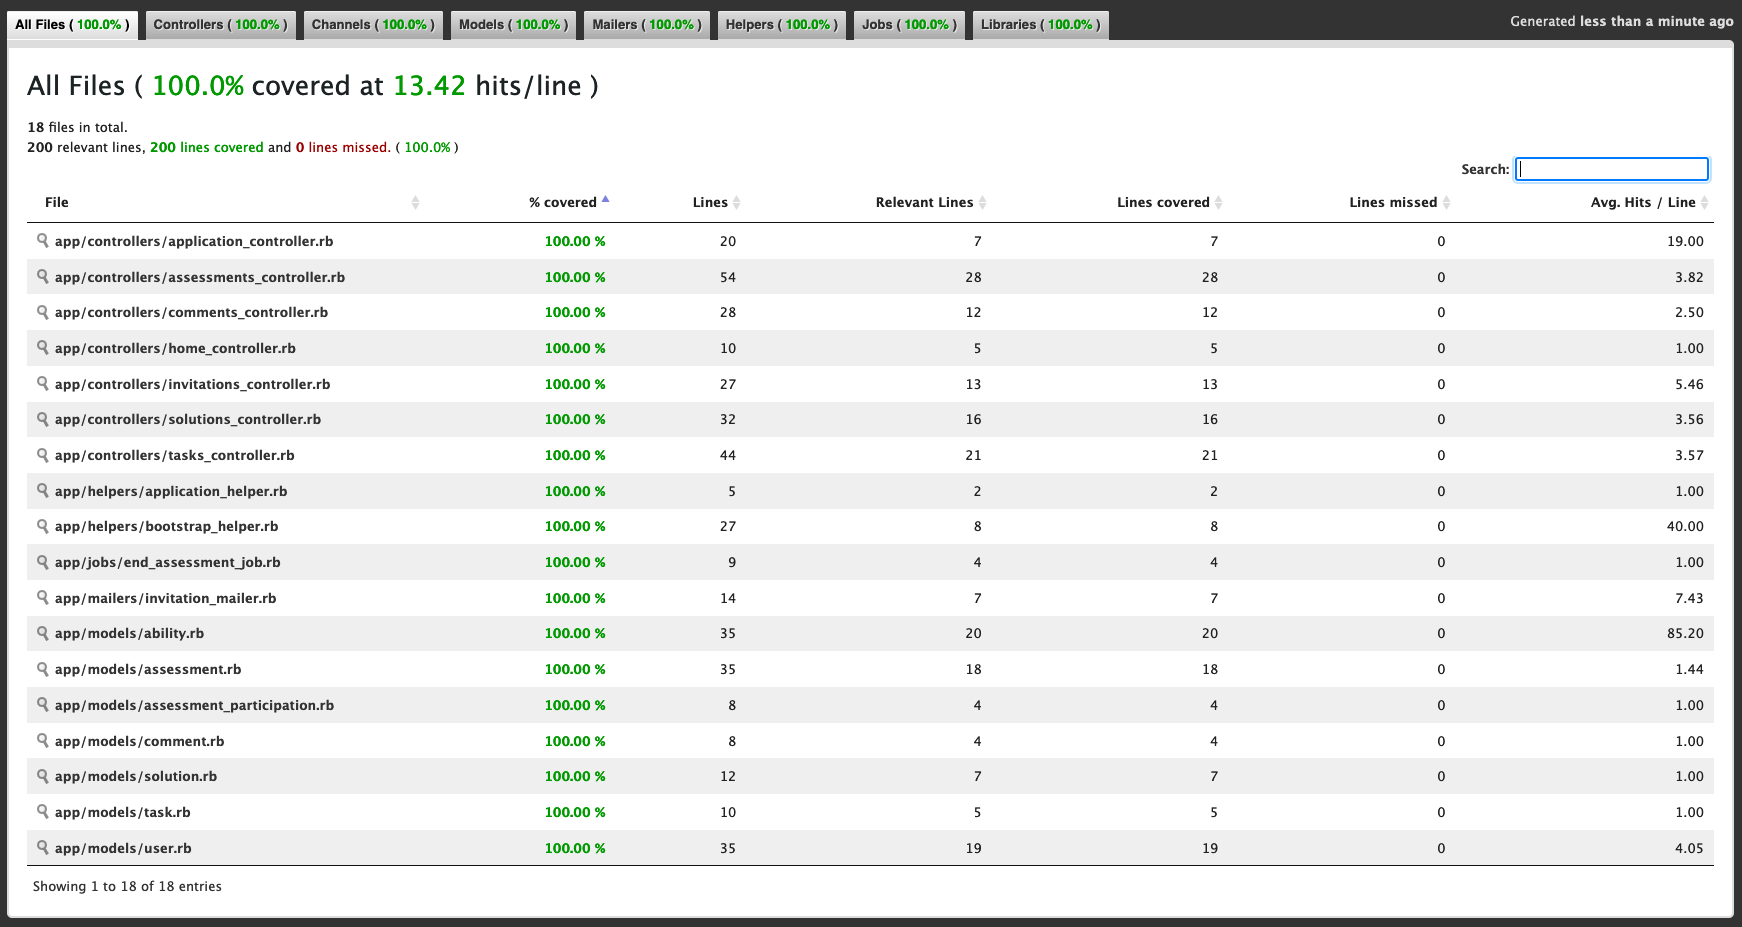
\includegraphics[width=\textwidth]{images/test-coverage.png}
  \caption{\label{fig:test-coverage}Erreichte \enquote{SimpleCov} Testabdeckung am 07.06.2022}
\end{figure}

Zusätzlich wurden planmässig alle Benutzer-Flows vollständig durch System-Tests gedeckt. Diese durchlaufen ebenfalls mit Erfolg und sind alle grün:

\begin{figure}[H]
  \centering
  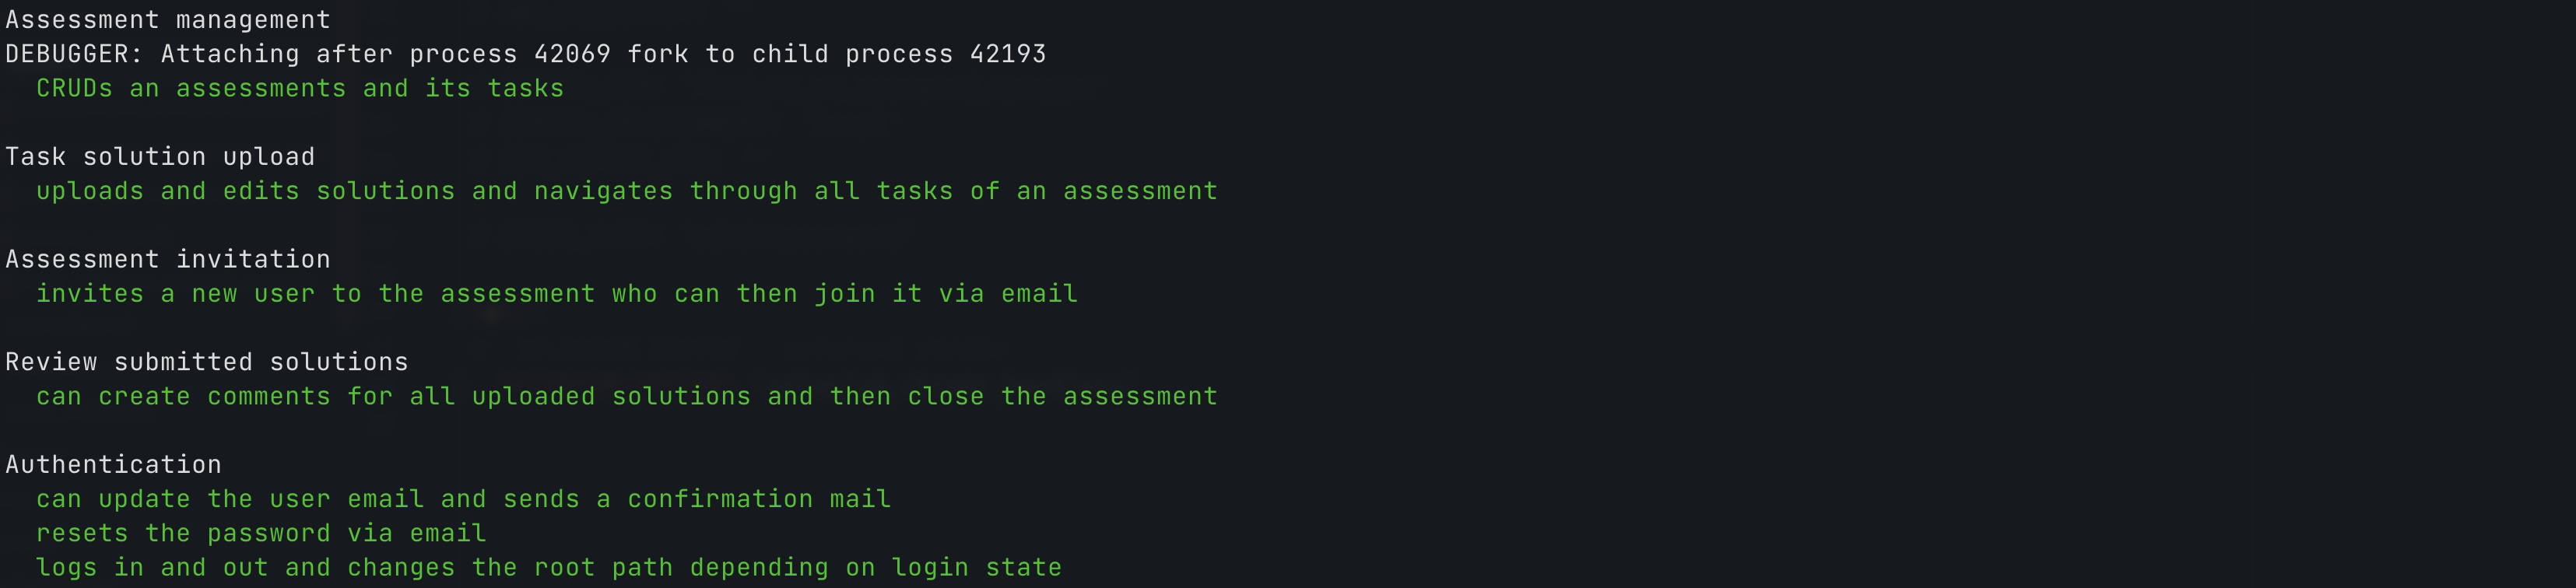
\includegraphics[width=\textwidth]{images/system-tests.png}
  \caption{\label{fig:system-tests}Durchlauf der Capybara System-Tets am 07.06.2022}
\end{figure}

\section{Linting-Checks}

Bei jedem CI-run werden nicht nur die oberhalb genannten automatisierten Tests ausgeführt, sondern der Code unterzieht sich auch diversen Linting- und Security-Checks.
Auch diese durchlaufen mit Erfolg und wurden an keiner Stelle im Code ignoriert. Damit entspricht der Ruby Code-Style in dieser PA vollständig den Rubocop-Guidelines.

\begin{figure}[H]
  \centering
  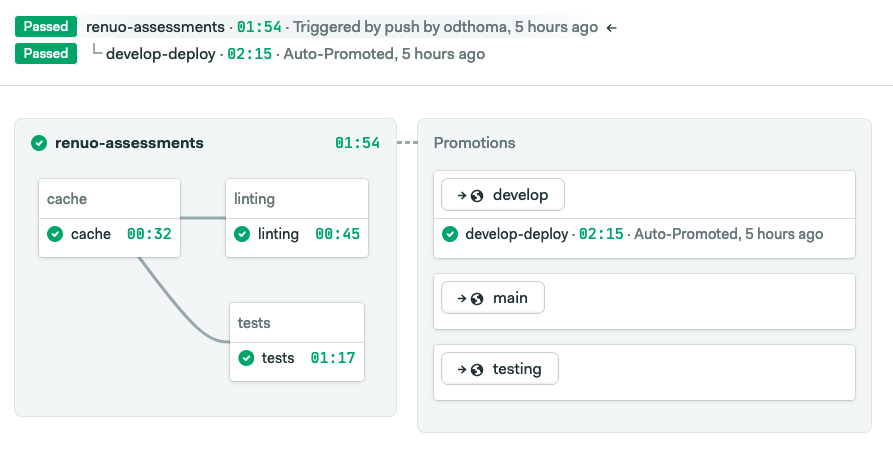
\includegraphics[width=\textwidth]{images/ci.png}
  \caption{\label{fig:semaphoreci}SemaphoreCI-Run vom letzten Git-Commit am 07.06.2022}
\end{figure}

\section{Manuelle Tests}

Auch die manuellen Tests konnten durch den Kandidaten, Oliver Thoma, mit Erfolg durchgeführt werden. Lediglich der Test \emph{ID 1} musste wiederholt werden, jedoch wurde beim zweiten Versuch
das erwartete Resultat erreicht. Ein korrektes Zusammenspiel aller Systeme auf der Produktions-Umgebung wurde somit sichergestellt.
Der Assessment-Assistant verhält sich dort nun genau so, wie auch schon auf der lokalen Umgebung des Kandidaten während der Entwicklungszeit.

\begin{table}[H]
  \begin{tabularx}{\linewidth}[H]{|c|l|l|X|}
    \hline
    \rowcolor{PrimaryColor!30} \textbf{Test-ID} & \textbf{Resultat} & \textbf{Datum und Uhrzeit} & \textbf{Bemerkungen}                                                                                          \\
    \hline
    1                                           & FAILED, SUCCESS   & 03.06.2022, 11:30 Uhr      & Dieser Test wurde aufgrund einer \gls{cors} Fehlkonfiguration auf der S3-development Instanz 2x durchgeführt. \\
    \hline
    2                                           & SUCCESS           & 06.06.2022, 13:30 Uhr      & Keine                                                                                                         \\
    \hline
    3                                           & SUCCESS           & 06.06.2022, 13:45 Uhr      & Keine                                                                                                         \\
    \hline
  \end{tabularx}
\end{table}
